% intensity
% spectral distribution
% solar geometry
% saules stāvoklis debesīs
% un virziens, kurā stara starojums krīt uz dažādu virzienu un ēnojuma virsmām

Lielākā daļa Saules emitētās enerģijas tiek saražota kodolreakcijās fotosfērā.

Saņemto enerģiju laika vienībā uz uz laukuma vienības perpendikulāri starojuma izplatīšanās virzienam 1 AU attālumā integrēta pa visiem viļņu garumiem raksturo solārā konstante ($G_{sc}$).



Solārā konstante $G_{sc}$ ir saņemtā enerģija laika vienībā uz laukuma vienības perpendikulāri starojuma izplatīšanās virzienam 1 AU attālumā integrēta pa visiem viļņu garumiem.\cite{ThermalProcesses}


Kaut gan absolūtais kopējais saules apstarojuma vērtība ir kontroversiāla, jo laika gaitā mērīta ar dažādiem radiometriem un kosmosa misijām, piemēram, 

\begin{table}[h]
    \caption{TSI mērījumu vēsture} % caption iet pirms tabulas
    \begin{center}
    \begin{tabular}{| r | c | l |}
    \hline
    radiometrs & misija & organizācija \\     \hline
    Hickey-Frieden & NIMBUS-7 & NOAA  \\     \hline
	ACRIM I & Solārā Maksimuma Misija (SMM) & NASA \\ 	\hline
	ACRIM  & Zemes Radiācijas Budžeta Satelīts (ERBS) & NASA \\ 	\hline
	ACRIM II & Augšējās Atmosfēras Izpētes Satelīts (UARS) & NASA \\ 	\hline
	VIRGO & Solārā un Heliosfēras observatorija (SOHO)& ESA/NASA \\ 	\hline
	ACRIM III & ACRIMSAT  & NASA \\ 	\hline
	TIM & Saules Radiācijas un Klimata Eksperiments (SORCE) & NASA \\
    \hline
    \end{tabular}
    \end{center}
    \label{tab:radiometers}
\end{table}




Kopējais saules apstarojums (TSI) ir saules starojuma absolūtās intensitātes mērījums integrēts visā saules enerģijas diskā un visā saules enerģijas spektrā.

diennakts vidējais apstarojums 1 AU attālumā no Saules.

Norāda uz solārās radiācijas izmaiņām, kas ietekmē solārās enerģijas apjomu uz Zemes atmosfēras augšējiem slāņiem.


Šajā darbā tiek izmantot TSI dati no SORCE (SOlar Radiation and Climate Experiment) TIM (Total Irradiance Montior) dati, pēc kuriem absolūtā vērtība ir $1360.8 \pm 0.5 \textrm{Wm}^{-2}$, jo tie ir precīzākie un ...\cite{Frohlich2012}

\begin{figure}[h]
    \centering
    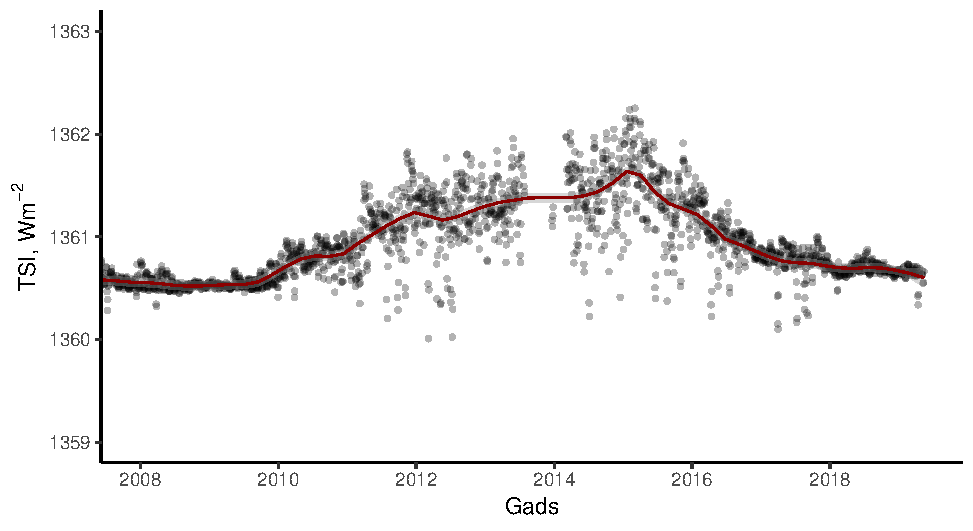
\includegraphics[width=\linewidth]{figures/misc/TSI_8-19.pdf}
    \caption{Kopējais saules apstarojums 24. saules ciklā}
    % \captionof{figure}{Kopējais saules apstarojums 24. saules ciklā}
    \label{fig:TSI1}
\end{figure}

\begin{figure}[h]
    \centering
    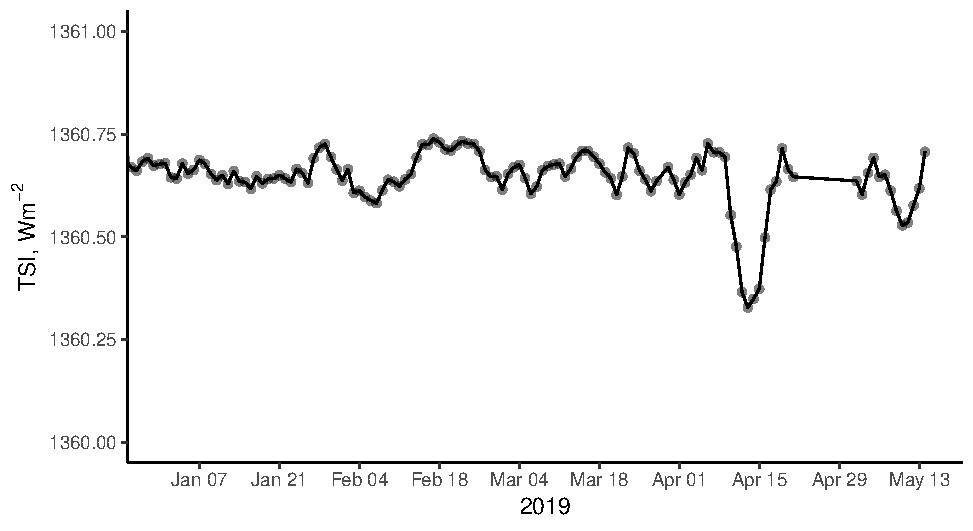
\includegraphics[width=\linewidth]{figures/misc/TSI.pdf}
    \caption{Kopējais saules apstarojums solāro paneļu datu ieguves laikā}
    % \captionof{figure}{Kopējais saules apstarojums solāro paneļu datu ieguves laikā}
    \label{fig:TSI2}
\end{figure}